\chapter*{My Extensions and Experiments}
\section*{Adjustments to the Original Code}
My work extends the code provided by the DRÆM paper \citep{zavrtanikDRAEMDiscriminativelyTrained2021}, mainly by additional anomaly generation methods\footnote{My full code is available at \url{https://github.com/christopher-rossbach/DRAEM_seminar_AD}.}.
To make full use of the HPC resources provided by NHR@FAU, I implemented micro-batch training and used automatic mixed precision (AMP) for the forward pass, while using full precision for loss calculation and evaluation to ensure numerical stability.
In addition to reducing the memory footprint, the implementation of micro-batches fixed a bug in the original code, where the last incomplete batch of each epoch was weighted incorrectly during training (see Figure~\ref{fig:smooth-loss-curve} in the appendix).
I also switched to a cosine annealing learning rate scheduler to ensure comparability between different methods without the need for additional hyperparameter searches.
These adjustments can be found in the \texttt{train\_DRAEM.py} script.
I performed multiple test runs after each adjustment to rule out any negative impact on the final performance.
In fact, my reproduced AUROC metrics (image- and pixel-level) on the combined MVTec dataset are within 0.1 percentage points of the values reported in the paper, while the pixel AP value improved from 68.4\% to 69.7\%, probably due to more stable training (average of 4 independent runs)\footnote{The metrics on a per-category basis differ notably more, but this can be attributed to the natural variance of the training process. For concrete values see Figure~\ref{fig:uniform_vs_poisson_perlin_all_metrics}.}.
The scripts for running the experiments with reproducible parametrization can be found in the \texttt{slurm} directory.

\begin{figure}[h]
    \centering
    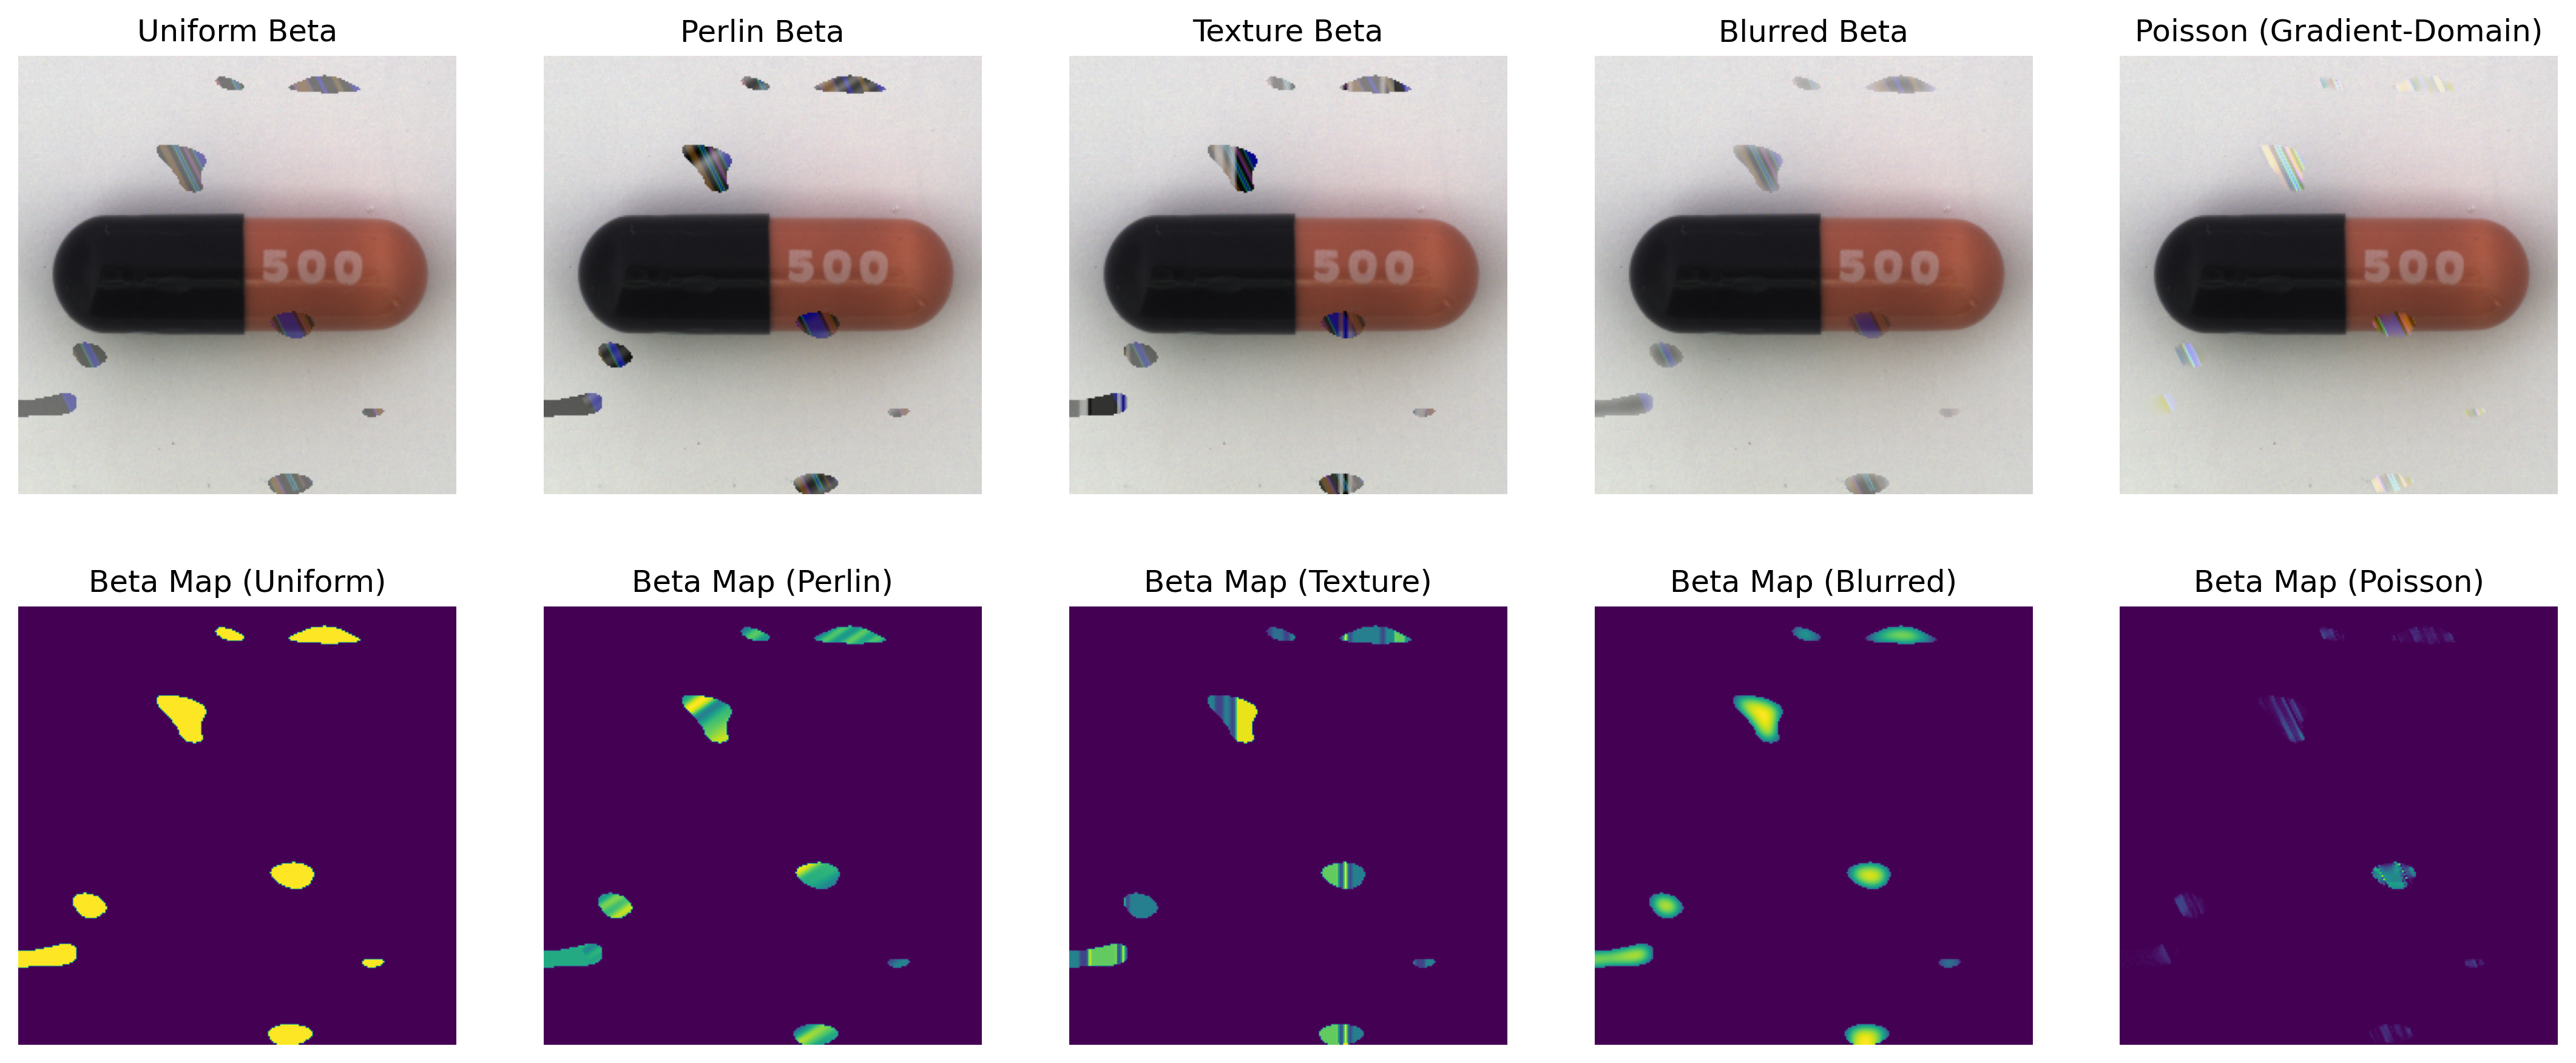
\includegraphics[width=\textwidth]{figures/blend-methods}
    \caption{Different blending methods (from left to right): uniform $\beta$, Perlin-$\beta$, texture-$\beta$, blurred $\beta$, Poisson image interpolation.
    The top row shows an example normal image with added anomalies.
    The bottom row shows the strength of the contribution of the anomaly to the final image.
    It is clearly visible how the anomaly strength in the Poisson image interpolation is guided by the image gradients (stronger near the edge of the pill).
    }
    \label{fig:blend-methods}
\end{figure}

\section*{Additional Blending Methods for Anomaly Generation}
My main contribution, implementing additional blending methods for anomaly generation, is part of the data loading pipeline and thus can be found in the \texttt{data\_loader.py} script.
I noted that the anomaly blending method in the paper always produced anomalies with sharp borders, which are arguably rather easy to spot.
By varying the anomaly strength throughout the anomaly region, more realistic anomalies can be generated, which should lead to a more robust model.
For all blending methods, I kept the original anomaly generation procedure, where a random anomaly mask is created by sampling and thresholding Perlin noise patterns and then applying the anomaly in the regions defined by the mask with a strength determined by the blending method.
The blending methods are: uniform $\beta$ blending (as in the original paper, without spatial variation in anomaly strength), Perlin-$\beta$ blending (where Perlin noise determines the anomaly opacity), texture-$\beta$ blending (where the luminance of a randomly sampled texture determines the anomaly opacity), blurred $\beta$ blending (where the borders of the anomaly mask are blurred), and channel-wise Poisson image interpolation, where the anomaly strength is guided by the source image gradient (see \citet{tanDetectingOutliersPoisson2021}\footnote{\citet{tanDetectingOutliersPoisson2021} also provides the interpolation code.}).
Examples of anomalies generated with these methods can be seen in Figure~\ref{fig:blend-methods}.
Performance numbers for these blending methods and their combinations are reported in Table~\ref{tab:ablation-blending}.
As can be seen, the Poisson image interpolation, as the only content-sensitive blending method, yields on average the best results\footnote{This method was suggested by my supervisor, Johanna Müller.}.
However, a closer look at the results reveals that, for some object categories, the other methods outperform the Poisson blending (see Figure~\ref{fig:blending_comparison_heatmap}).
Combining the Poisson blending with other methods during training leverages these mutual benefits and leads to the best overall performance (last row in Table~\ref{tab:ablation-blending}).
The combination of methods was implemented by randomly selecting one blending method for each training image.
A full excerpt of the performance metrics can be found in the appendix.

\begin{table}[h]
    \centering
                \begin{tabular}{lccc}
                \hline
                \textbf{Method} & \textbf{Image AUROC} $\uparrow$ & \textbf{Pixel AUROC} $\uparrow$ & \textbf{Pixel AP} $\uparrow$ \\
                \hline
                DRÆM-Uniform & \cellcolor[HTML]{E3F399} 98.0\% & \cellcolor[HTML]{BFE47A} 97.3\% & \cellcolor[HTML]{FFFEBE} 69.7\% \\
                DRÆM-Blurred & \cellcolor[HTML]{A50026} 96.4\% & \cellcolor[HTML]{A50026} 96.0\% & \cellcolor[HTML]{A50026} 65.8\% \\
                DRÆM-Texture & \cellcolor[HTML]{E3F399} 98.0\% & \cellcolor[HTML]{D9EF8B} 97.2\% & \cellcolor[HTML]{FEE797} 69.1\% \\
                DRÆM-Perlin & \cellcolor[HTML]{C3E67D} 98.2\% & \cellcolor[HTML]{BFE47A} 97.3\% & \cellcolor[HTML]{FFF7B2} 69.5\% \\
                DRÆM-Poisson & \cellcolor[HTML]{097940} \underline{99.1\%} & \cellcolor[HTML]{199750} \underline{97.8\%} & \cellcolor[HTML]{89CC67} \underline{71.6\%} \\
                DRÆM-Poisson+Perlin & \cellcolor[HTML]{006837} \textbf{99.2\%} & \cellcolor[HTML]{006837} \textbf{98.0\%} & \cellcolor[HTML]{006837} \textbf{73.6\%} \\
                \hline
            \end{tabular}
    \caption{Key performance metrics (image-level AUROC, pixel-level AUROC, pixel-level AP) on the combined MVTec dataset for different blending methods used.}
    \label{tab:ablation-blending}
\end{table}


%Things that I want to mention:
%\begin{itemize}
    %\item[\checkmark] Micro-batch implementation
    %\item[\checkmark] github repo linken
    %\item Code organisation (verschiedene dateien)
    %\item[\checkmark] Verwendung von Cosine Annealing Scheduler (Vergleichbarkeit)
    %\item[\checkmark] AMP
    %\item[\checkmark] Neu implementierte Blendings
    %\item[\checkmark] kopierter code fuer Poisson Image Interpolation (channel wise)
    %\item[\checkmark] Uebereinstimmung eigener Durchschnittswerte mit paper
    %\item[\checkmark] Abweichung eigener reproduzierter werte von paper
    %\item[\checkmark] Slurm scripte
    %\item[\checkmark] 4 runs per config
    %\item[\checkmark] Motivation kombinierte configs (mututal benefits)
    %\item 
%\end{itemize}